\documentclass{standalone}
\usepackage{tikz}
\usetikzlibrary{patterns, positioning}


\begin{document}
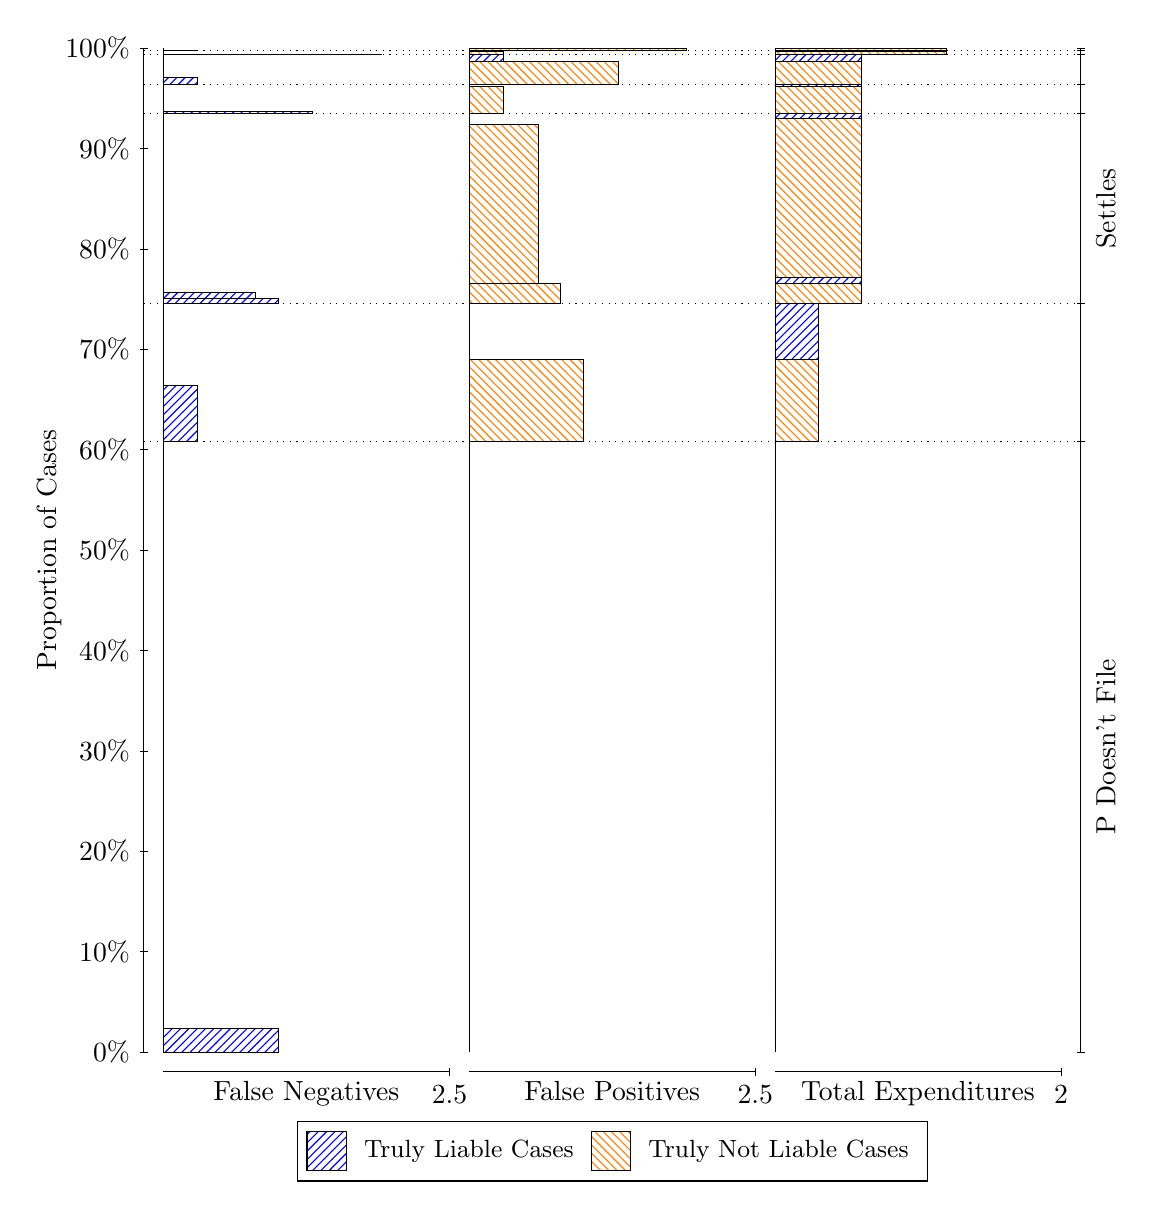
\begin{tikzpicture}
\draw[black, very thin] (1.5,1.75) -- (1.5,14.5);
\node[rotate=90, text=black, anchor=center] at (0.3, 8.125) {Proportion of Cases};
\draw[black, very thin] (1.45,1.75) -- (1.55,1.75);
\node[text=black, anchor=east] at (1.45, 1.75) {0\%};
\draw[black, very thin] (1.45,3.025) -- (1.55,3.025);
\node[text=black, anchor=east] at (1.45, 3.025) {10\%};
\draw[black, very thin] (1.45,4.3) -- (1.55,4.3);
\node[text=black, anchor=east] at (1.45, 4.3) {20\%};
\draw[black, very thin] (1.45,5.575) -- (1.55,5.575);
\node[text=black, anchor=east] at (1.45, 5.575) {30\%};
\draw[black, very thin] (1.45,6.85) -- (1.55,6.85);
\node[text=black, anchor=east] at (1.45, 6.85) {40\%};
\draw[black, very thin] (1.45,8.125) -- (1.55,8.125);
\node[text=black, anchor=east] at (1.45, 8.125) {50\%};
\draw[black, very thin] (1.45,9.4) -- (1.55,9.4);
\node[text=black, anchor=east] at (1.45, 9.4) {60\%};
\draw[black, very thin] (1.45,10.675) -- (1.55,10.675);
\node[text=black, anchor=east] at (1.45, 10.675) {70\%};
\draw[black, very thin] (1.45,11.95) -- (1.55,11.95);
\node[text=black, anchor=east] at (1.45, 11.95) {80\%};
\draw[black, very thin] (1.45,13.225) -- (1.55,13.225);
\node[text=black, anchor=east] at (1.45, 13.225) {90\%};
\draw[black, very thin] (1.45,14.5) -- (1.55,14.5);
\node[text=black, anchor=east] at (1.45, 14.5) {100\%};

\draw[black, very thin] (13.4,1.75) -- (13.4,14.5);
\draw[black, very thin] (13.35,1.75) -- (13.45,1.75);
\node[anchor=west] at (13.35, 1.75) {};
\draw[black, very thin] (13.35,9.5) -- (13.45,9.5);
\node[anchor=west] at (13.35, 9.5) {};
\draw[black, very thin] (13.35,11.257) -- (13.45,11.257);
\node[anchor=west] at (13.35, 11.257) {};
\draw[black, very thin] (13.35,13.671) -- (13.45,13.671);
\node[anchor=west] at (13.35, 13.671) {};
\draw[black, very thin] (13.35,14.037) -- (13.45,14.037);
\node[anchor=west] at (13.35, 14.037) {};
\draw[black, very thin] (13.35,14.415) -- (13.45,14.415);
\node[anchor=west] at (13.35, 14.415) {};
\draw[black, very thin] (13.35,14.468) -- (13.45,14.468);
\node[anchor=west] at (13.35, 14.468) {};
\draw[black, very thin] (13.35,14.5) -- (13.45,14.5);
\node[anchor=west] at (13.35, 14.5) {};

\draw[black, very thin, pattern color=blue, pattern=north east lines] (1.75,1.75) rectangle (3.2033,2.0453);
\draw[black, very thin, pattern color=orange, pattern=north west lines] (1.75,2.0453) rectangle (1.75,9.5);
\draw[black, very thin, pattern color=blue, pattern=north east lines] (1.75,9.5) rectangle (2.186,10.213);
\draw[black, very thin, pattern color=orange, pattern=north west lines] (1.75,10.213) rectangle (1.75,11.257);
\draw[black, very thin, pattern color=blue, pattern=north east lines] (1.75,11.257) rectangle (3.2033,11.322);
\draw[black, very thin, pattern color=blue, pattern=north east lines] (1.75,11.322) rectangle (2.9127,11.401);
\draw[black, very thin, pattern color=orange, pattern=north west lines] (1.75,11.401) rectangle (1.75,13.671);
\draw[black, very thin, pattern color=blue, pattern=north east lines] (1.75,13.671) rectangle (3.6393,13.696);
\draw[black, very thin, pattern color=orange, pattern=north west lines] (1.75,13.696) rectangle (1.75,14.037);
\draw[black, very thin, pattern color=blue, pattern=north east lines] (1.75,14.037) rectangle (2.186,14.126);
\draw[black, very thin, pattern color=orange, pattern=north west lines] (1.75,14.126) rectangle (1.75,14.415);
\draw[black, very thin, pattern color=blue, pattern=north east lines] (1.75,14.415) rectangle (4.5113,14.417);
\draw[black, very thin, pattern color=orange, pattern=north west lines] (1.75,14.417) rectangle (1.75,14.468);
\draw[black, very thin, pattern color=blue, pattern=north east lines] (1.75,14.468) rectangle (2.186,14.474);
\draw[black, very thin, pattern color=orange, pattern=north west lines] (1.75,14.474) rectangle (1.75,14.5);
\draw[black, very thin, pattern color=orange, pattern=north west lines] (5.6333,1.75) rectangle (5.6333,9.2048);
\draw[black, very thin, pattern color=blue, pattern=north east lines] (5.6333,9.2048) rectangle (5.6333,9.5);
\draw[black, very thin, pattern color=orange, pattern=north west lines] (5.6333,9.5) rectangle (7.0867,10.544);
\draw[black, very thin, pattern color=blue, pattern=north east lines] (5.6333,10.544) rectangle (5.6333,11.257);
\draw[black, very thin, pattern color=orange, pattern=north west lines] (5.6333,11.257) rectangle (6.796,11.509);
\draw[black, very thin, pattern color=orange, pattern=north west lines] (5.6333,11.509) rectangle (6.5053,13.527);
\draw[black, very thin, pattern color=blue, pattern=north east lines] (5.6333,13.527) rectangle (5.6333,13.671);
\draw[black, very thin, pattern color=orange, pattern=north west lines] (5.6333,13.671) rectangle (6.0693,14.011);
\draw[black, very thin, pattern color=blue, pattern=north east lines] (5.6333,14.011) rectangle (5.6333,14.037);
\draw[black, very thin, pattern color=orange, pattern=north west lines] (5.6333,14.037) rectangle (7.5227,14.326);
\draw[black, very thin, pattern color=blue, pattern=north east lines] (5.6333,14.326) rectangle (6.0693,14.415);
\draw[black, very thin, pattern color=orange, pattern=north west lines] (5.6333,14.415) rectangle (6.0693,14.465);
\draw[black, very thin, pattern color=blue, pattern=north east lines] (5.6333,14.465) rectangle (5.6333,14.468);
\draw[black, very thin, pattern color=orange, pattern=north west lines] (5.6333,14.468) rectangle (8.3947,14.494);
\draw[black, very thin, pattern color=blue, pattern=north east lines] (5.6333,14.494) rectangle (6.9413,14.5);
\draw[black, very thin, pattern color=orange, pattern=north west lines] (9.5167,1.75) rectangle (9.5167,9.2048);
\draw[black, very thin, pattern color=blue, pattern=north east lines] (9.5167,9.2048) rectangle (9.5167,9.5);
\draw[black, very thin, pattern color=orange, pattern=north west lines] (9.5167,9.5) rectangle (10.062,10.544);
\draw[black, very thin, pattern color=blue, pattern=north east lines] (9.5167,10.544) rectangle (10.062,11.257);
\draw[black, very thin, pattern color=orange, pattern=north west lines] (9.5167,11.257) rectangle (10.607,11.509);
\draw[black, very thin, pattern color=blue, pattern=north east lines] (9.5167,11.509) rectangle (10.607,11.587);
\draw[black, very thin, pattern color=orange, pattern=north west lines] (9.5167,11.587) rectangle (10.607,13.606);
\draw[black, very thin, pattern color=blue, pattern=north east lines] (9.5167,13.606) rectangle (10.607,13.671);
\draw[black, very thin, pattern color=orange, pattern=north west lines] (9.5167,13.671) rectangle (10.607,14.011);
\draw[black, very thin, pattern color=blue, pattern=north east lines] (9.5167,14.011) rectangle (10.607,14.037);
\draw[black, very thin, pattern color=orange, pattern=north west lines] (9.5167,14.037) rectangle (10.607,14.326);
\draw[black, very thin, pattern color=blue, pattern=north east lines] (9.5167,14.326) rectangle (10.607,14.415);
\draw[black, very thin, pattern color=orange, pattern=north west lines] (9.5167,14.415) rectangle (11.697,14.465);
\draw[black, very thin, pattern color=blue, pattern=north east lines] (9.5167,14.465) rectangle (11.697,14.468);
\draw[black, very thin, pattern color=orange, pattern=north west lines] (9.5167,14.468) rectangle (11.697,14.494);
\draw[black, very thin, pattern color=blue, pattern=north east lines] (9.5167,14.494) rectangle (11.697,14.5);
\draw[black, dotted] (1.5,9.5) -- (13.4,9.5);
\draw[black, dotted] (1.5,11.257) -- (13.4,11.257);
\draw[black, dotted] (1.5,13.671) -- (13.4,13.671);
\draw[black, dotted] (1.5,14.037) -- (13.4,14.037);
\draw[black, dotted] (1.5,14.415) -- (13.4,14.415);
\draw[black, dotted] (1.5,14.468) -- (13.4,14.468);
\draw[black, very thin] (1.75,1.5) -- (5.3833,1.5);
\node[text=black, anchor=north] at (3.5667, 1.5) {False Negatives};
\draw[black, very thin] (5.3833,1.45) -- (5.3833,1.55);
\node[text=black, anchor=north] at (5.3833, 1.45) {2.5};

\draw[black, very thin] (5.6333,1.5) -- (9.2667,1.5);
\node[text=black, anchor=north] at (7.45, 1.5) {False Positives};
\draw[black, very thin] (9.2667,1.45) -- (9.2667,1.55);
\node[text=black, anchor=north] at (9.2667, 1.45) {2.5};

\draw[black, very thin] (9.5167,1.5) -- (13.15,1.5);
\node[text=black, anchor=north] at (11.333, 1.5) {Total Expenditures};
\draw[black, very thin] (13.15,1.45) -- (13.15,1.55);
\node[text=black, anchor=north] at (13.15, 1.45) {2};

\node[text=black, centered, rotate=90] at (13.72, 5.625) {P Doesn't File};

\node[text=black, centered, rotate=90] at (13.72, 12.464) {Settles};





\draw (7.449999999999999,1.5) node[draw=none] (baseCoordinate) {};
\begin{scope}[align=center]
        \matrix[scale=0.5, draw=black, below=0.5cm of baseCoordinate, nodes={draw}, column sep=0.1cm]{
            \node[rectangle, draw, minimum width=0.5cm, minimum height=0.5cm, pattern color=blue, pattern=north east lines] {}; &
            \node[draw=none, font=\small, text=black] (B) {Truly Liable Cases}; &
            \node[rectangle, draw, minimum width=0.5cm, minimum height=0.5cm, pattern color=orange, pattern=north west lines] {}; &
            \node[draw=none, font=\small, text=black] (B) {Truly Not Liable Cases}; \\
            };
\end{scope}

\end{tikzpicture}
\end{document}